\documentclass{article}
\usepackage{amsmath}
\usepackage{amssymb}
\usepackage[hmargin=1.8cm,vmargin=2.5cm]{geometry}
\usepackage{tabularx}
\usepackage{booktabs}
\usepackage{graphicx}
\usepackage{color}
\usepackage{wrapfig}
\usepackage{multirow}
\usepackage{multicol}
\usepackage{cite}
\usepackage[rightcaption]{sidecap}
%\usepackage{hyperref}
\usepackage{threeparttable}
\usepackage[table]{xcolor}
\usepackage{psfrag}
\usepackage[margin=10pt,font=small,textfont=sf,labelfont=bf]{caption}
\usepackage{subfig}
\usepackage[section]{placeins}

\title{NbTi Side Coax Stresses}
\author{Nicholas Kellaris}
\begin{document}
\bibliographystyle{plain}
\maketitle

\section{Tower Model for Contraction Lengths}

\begin{figure}[h]
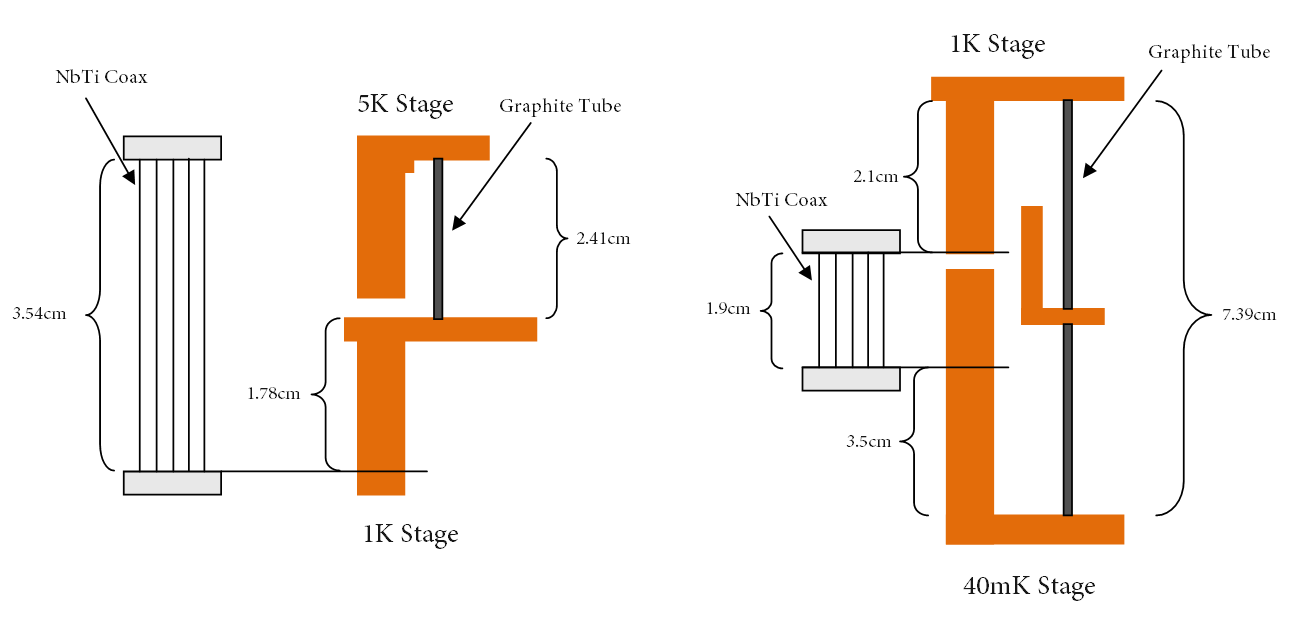
\includegraphics[width = \textwidth]{Contraction_diagram.png}
\caption{The following tower model was used in considering the relative contractions of the tower components.}
\end{figure}

The above tower model was used to determine the tensile stress on the side coaxes. These models consider the contiguous structure supporting the NbTi side coaxes, and its length change. This is compared to the length change of the NbTi wires.

\section{Stress on 5K - 1K Span Coax}

To calculate the stress on the NbTi wires, the strain was first calculated. Referring to Figure 1, we see that the contiguous structure supporting the side coax consists of 2.41cm of graphite tube and 1.78cm of copper. The contraction of these will bring the ends of the wire closer together, decreasing strain. Conversely, the 3.54cm of NbTi wire will contract, acting to increase the strain. A third factor which comes into play is the tension created in the wire during the construction of the side coax. Combining all these effects, we calculate the wire length at 4K and compare it to the equilibrium length. This gives a strain which can be translated into a stress.

\newpage
\section{Coefficients of Thermal Expansion}

Using NIST's database, the temperature-dependent CTE of OFHC Copper was found. This is shown in figure 2 to the right.

\begin{wrapfigure}{r}{9cm}
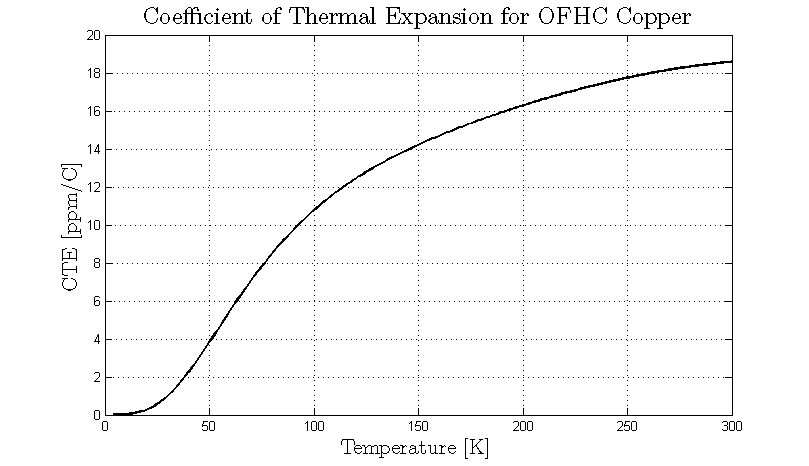
\includegraphics[width = .5\textwidth]{CTE_Copper_plot.png}
\end{wrapfigure} 

The equation for thermal contraction could then be integrated from 300K to 4K (the lowest data range for the equation) to get total fractional contraction. 

The contraction of NbTi was found differently from copper. An equation for integrated thermal contraction was used, rather than one for just the coefficient. This equation reads,
$$
\frac{L_{T} - L_{300}}{L_{300}} = (a + bT + cT^2 + dT^3 + eT^4) \cdot 10^{-5}
$$
where a,b,c,d,e are a measured set of coefficients. 

The CTE for UF-4S graphite was obtained from a data sheet provided by Mersen, and is not given as a function of temperature. The CTE for UF-4S graphite is low, and depends on the grain orientation:
$$
CTE_{\parallel} = 1.8 \cdot 10^{-6}/C 
$$
$$
CTE_{\perp} = 2.9 \cdot 10^{-6}/C
$$
where $CTE_{\parallel}$ is measured with the grain, and $CTE_{\perp}$ against the grain. The lower value of CTE is used in the calculations that follow, as a safety buffer.

\subsection{Tension from Fabrication}

The NbTi wires are soldered under tension to prevent loss of tension (and shorts) at operation temperature. This is done with two 30g weights - one hung at either end - for a total of 60g. Dividing by the cross-section of the wires, we get a stress of $805MPa$. The Modulus of Elasticity, $E$, for our Nb-47Ti (47\% Ti by weight) is $75.15GPa$. Using this, we get a strain of,
$$
Strain = \frac{Stress}{E} = \frac{75.15e9}{805e6} = 0.0107 \ or \ 1.07\%
$$

so the wires are tensioned 1.07\% beyond their equilibrium length.

\subsection{Total Stress and Strain at 4K}
The strain is calculated from 
$$
Strain = \frac{L - L_{eq}}{L_{eq}}
$$
where $L$ is the actual length of the wires and $L_{eq}$ is the equilibrium length at 4K. We can see that 
$$ 
L = L_{NbTi} - |\Delta L_{Cu}| - |\Delta L_{Tube}|
$$
while,
$$
L_{eq} = L_{NbTi} \cdot (1 - 0.0107 - |\Delta L_{NbTi}|)
$$ 
where $\Delta L_{Cu}$ is the total contraction of the copper whose length is given in figure 1, $\Delta L_{Tube}$, is the graphite tube contraction, $\Delta L_{NbTi}$ is the NbTi contraction, and $L_{NbTi}$ is the original length of the wires at 300K (3.54cm in this case). Multiplying by $1 - 0.0107$ gives the length at 300K without the fabrication tension. Putting these into the strain equation gives $1.05 \%$ strain. From this we find,
$$
Stress = E \cdot Strain = 75.15e9 \cdot 0.0105 = 791MPa
$$

\section{Stress on 1K - 40mK Span Coax}

The analysis carried out for the 1K - 40mK cable is similar to that for the 5K - 1K cable. For this cable, the contiguous support structure is more complicated. First, we have 7.39cm of graphite tube which will act to bring the wire ends closer together, decreasing strain. Second, we have the contracting copper. Due to the design of the tower (coax solder attachment points, etc.) we actually have $2.1cm + 3.5cm = 5.6cm$ of copper whose contraction will act to increase strain. Third, we have the contraction of the NbTi wires themselves, acting to increase the strain. Finally, we have the same applied tension at before, which increases strain by the same 1.07\%.

\subsection{Total Stress and Strain at 4K}
The strain is still calculated from
$$
Strain = \frac{L - L_{eq}}{L_{eq}}
$$

For this span, however, we will have,
$$
L = L_{NbTi} + |\Delta L_{Cu}| - |\Delta L_{Tube}|
$$
where the sign change in front of $|\Delta L_{Cu}|$ reflects the tendency to increase separation in this case. As before, we have,
$$
L_{eq} = L_{NbTi} \cdot (1 - 0.0107 - |\Delta L_{NbTi}|)
$$
with the same designations as before. Putting these into the strain equation gives $\approx 2.13 \%$ strain. This will be slightly less (about $2\%$) if the low CTE for graphite is used. From this we find,
$$
Stress = E \cdot Strain = 75.15e9 \cdot 0.0105 = 1604MPa
$$

This stress is much higher than the 5K - 1K coax stress. This is expected due to the short length of the wires for this span, as well as the large length of copper which is contracting. Though there is also a large length of graphite, its low CTE means it won't affect the total stress significantly.

\end{document}
